% Options for packages loaded elsewhere
\PassOptionsToPackage{unicode}{hyperref}
\PassOptionsToPackage{hyphens}{url}
%
\documentclass[
]{article}
\usepackage{lmodern}
\usepackage{amssymb,amsmath}
\usepackage{ifxetex,ifluatex}
\ifnum 0\ifxetex 1\fi\ifluatex 1\fi=0 % if pdftex
  \usepackage[T1]{fontenc}
  \usepackage[utf8]{inputenc}
  \usepackage{textcomp} % provide euro and other symbols
\else % if luatex or xetex
  \usepackage{unicode-math}
  \defaultfontfeatures{Scale=MatchLowercase}
  \defaultfontfeatures[\rmfamily]{Ligatures=TeX,Scale=1}
\fi
% Use upquote if available, for straight quotes in verbatim environments
\IfFileExists{upquote.sty}{\usepackage{upquote}}{}
\IfFileExists{microtype.sty}{% use microtype if available
  \usepackage[]{microtype}
  \UseMicrotypeSet[protrusion]{basicmath} % disable protrusion for tt fonts
}{}
\makeatletter
\@ifundefined{KOMAClassName}{% if non-KOMA class
  \IfFileExists{parskip.sty}{%
    \usepackage{parskip}
  }{% else
    \setlength{\parindent}{0pt}
    \setlength{\parskip}{6pt plus 2pt minus 1pt}}
}{% if KOMA class
  \KOMAoptions{parskip=half}}
\makeatother
\usepackage{xcolor}
\IfFileExists{xurl.sty}{\usepackage{xurl}}{} % add URL line breaks if available
\IfFileExists{bookmark.sty}{\usepackage{bookmark}}{\usepackage{hyperref}}
\hypersetup{
  pdftitle={Proyecto},
  hidelinks,
  pdfcreator={LaTeX via pandoc}}
\urlstyle{same} % disable monospaced font for URLs
\usepackage[margin=1in]{geometry}
\usepackage{color}
\usepackage{fancyvrb}
\newcommand{\VerbBar}{|}
\newcommand{\VERB}{\Verb[commandchars=\\\{\}]}
\DefineVerbatimEnvironment{Highlighting}{Verbatim}{commandchars=\\\{\}}
% Add ',fontsize=\small' for more characters per line
\usepackage{framed}
\definecolor{shadecolor}{RGB}{248,248,248}
\newenvironment{Shaded}{\begin{snugshade}}{\end{snugshade}}
\newcommand{\AlertTok}[1]{\textcolor[rgb]{0.94,0.16,0.16}{#1}}
\newcommand{\AnnotationTok}[1]{\textcolor[rgb]{0.56,0.35,0.01}{\textbf{\textit{#1}}}}
\newcommand{\AttributeTok}[1]{\textcolor[rgb]{0.77,0.63,0.00}{#1}}
\newcommand{\BaseNTok}[1]{\textcolor[rgb]{0.00,0.00,0.81}{#1}}
\newcommand{\BuiltInTok}[1]{#1}
\newcommand{\CharTok}[1]{\textcolor[rgb]{0.31,0.60,0.02}{#1}}
\newcommand{\CommentTok}[1]{\textcolor[rgb]{0.56,0.35,0.01}{\textit{#1}}}
\newcommand{\CommentVarTok}[1]{\textcolor[rgb]{0.56,0.35,0.01}{\textbf{\textit{#1}}}}
\newcommand{\ConstantTok}[1]{\textcolor[rgb]{0.00,0.00,0.00}{#1}}
\newcommand{\ControlFlowTok}[1]{\textcolor[rgb]{0.13,0.29,0.53}{\textbf{#1}}}
\newcommand{\DataTypeTok}[1]{\textcolor[rgb]{0.13,0.29,0.53}{#1}}
\newcommand{\DecValTok}[1]{\textcolor[rgb]{0.00,0.00,0.81}{#1}}
\newcommand{\DocumentationTok}[1]{\textcolor[rgb]{0.56,0.35,0.01}{\textbf{\textit{#1}}}}
\newcommand{\ErrorTok}[1]{\textcolor[rgb]{0.64,0.00,0.00}{\textbf{#1}}}
\newcommand{\ExtensionTok}[1]{#1}
\newcommand{\FloatTok}[1]{\textcolor[rgb]{0.00,0.00,0.81}{#1}}
\newcommand{\FunctionTok}[1]{\textcolor[rgb]{0.00,0.00,0.00}{#1}}
\newcommand{\ImportTok}[1]{#1}
\newcommand{\InformationTok}[1]{\textcolor[rgb]{0.56,0.35,0.01}{\textbf{\textit{#1}}}}
\newcommand{\KeywordTok}[1]{\textcolor[rgb]{0.13,0.29,0.53}{\textbf{#1}}}
\newcommand{\NormalTok}[1]{#1}
\newcommand{\OperatorTok}[1]{\textcolor[rgb]{0.81,0.36,0.00}{\textbf{#1}}}
\newcommand{\OtherTok}[1]{\textcolor[rgb]{0.56,0.35,0.01}{#1}}
\newcommand{\PreprocessorTok}[1]{\textcolor[rgb]{0.56,0.35,0.01}{\textit{#1}}}
\newcommand{\RegionMarkerTok}[1]{#1}
\newcommand{\SpecialCharTok}[1]{\textcolor[rgb]{0.00,0.00,0.00}{#1}}
\newcommand{\SpecialStringTok}[1]{\textcolor[rgb]{0.31,0.60,0.02}{#1}}
\newcommand{\StringTok}[1]{\textcolor[rgb]{0.31,0.60,0.02}{#1}}
\newcommand{\VariableTok}[1]{\textcolor[rgb]{0.00,0.00,0.00}{#1}}
\newcommand{\VerbatimStringTok}[1]{\textcolor[rgb]{0.31,0.60,0.02}{#1}}
\newcommand{\WarningTok}[1]{\textcolor[rgb]{0.56,0.35,0.01}{\textbf{\textit{#1}}}}
\usepackage{graphicx}
\makeatletter
\def\maxwidth{\ifdim\Gin@nat@width>\linewidth\linewidth\else\Gin@nat@width\fi}
\def\maxheight{\ifdim\Gin@nat@height>\textheight\textheight\else\Gin@nat@height\fi}
\makeatother
% Scale images if necessary, so that they will not overflow the page
% margins by default, and it is still possible to overwrite the defaults
% using explicit options in \includegraphics[width, height, ...]{}
\setkeys{Gin}{width=\maxwidth,height=\maxheight,keepaspectratio}
% Set default figure placement to htbp
\makeatletter
\def\fps@figure{htbp}
\makeatother
\setlength{\emergencystretch}{3em} % prevent overfull lines
\providecommand{\tightlist}{%
  \setlength{\itemsep}{0pt}\setlength{\parskip}{0pt}}
\setcounter{secnumdepth}{-\maxdimen} % remove section numbering

\title{Proyecto}
\author{}
\date{\vspace{-2.5em}2022-05-10}

\begin{document}
\maketitle

\hypertarget{r-markdown}{%
\subsection{R Markdown}\label{r-markdown}}

Cargamos los datos:

\begin{Shaded}
\begin{Highlighting}[]
\NormalTok{info \textless{}{-}}\StringTok{ }\KeywordTok{read.csv}\NormalTok{(}\StringTok{\textquotesingle{}data/datosfinales.csv\textquotesingle{}}\NormalTok{)}
\end{Highlighting}
\end{Shaded}

\hypertarget{planteamiento-del-problema}{%
\subsection{Planteamiento del
problema}\label{planteamiento-del-problema}}

La Ciudad de México es una de las 10 ciudades más grandes del mundo por
población con habitantes al 2020, sin contar la zona metropolitana que
incluye zonas del Estado de México e Hidalgo. Una población de este
tamaño exige un sistema de transporte público masivo de alta frecuencia,
volumen y disponibilidad. El sistema de transporte público unificado en
la Ciudad de México es en nuestra opinión uno relativamente bien
planeado y accesible. Sin embargo, como personas que no vivimos en la
periferia de la zona metropolitana nuestras opiniones pueden estar
sesgadas.

El objetivo de esta investigación es cuantificar el nivel de acceso de
la población de distintas alcaldías de la ciudad a los diversos medios
de transporte público masivo. Como transporte público masivo estamos
tomando en cuenta los siguientes servicios de transporte unificado que
ofrece la ciudad:

\begin{itemize}
\tightlist
\item
  Metro
\item
  Metrobus
\item
  Tren Ligero
\item
  Cablebus
\end{itemize}

Elegimos concentrarnos en estos servicios por las siguientes
características:

\begin{enumerate}
\def\labelenumi{\arabic{enumi}.}
\item
  Frecuencia. La frecuencia con la que pasan nuevos convoyes debe ser
  relativamente alta. Por ejemplo, en horas pico pasan convoyes nuevos
  de metro y metrobus en pocos minutos.
\item
  Volumen. Nos concentramos en transportes de alto volumen, excluyendo
  peseros y microbuses.
\item
  Unificado. Nos concentramos en el sistema de transporte unificado
  coordinado por el gobierno de la Ciudad de México.
\end{enumerate}

Además de hacer una exploración el objetivo de esta investigación es
determinar que tan bien distribuido está el transporte público en la
ciudad. Como habitantes de la CDMX tenemos la sospecha de que el
transporte público está muy centralizado en la zona del centro
histórico. Es decir, sospechamos que el sistema de transporte público
privilegia a las personas que viven en las delegaciones como Benito
Juárez, Cuauhtémoc, etc\ldots{} que no son necesariamente las
delegaciones con las poblaciones más altas.

Estas relaciones las exploraremos mediante diversas técnicas cubiertas
en el curso. Primero que nada procedemos con análisis exploratorio para
empezar a ganar intuición sobre el conjunto de datos. Más tarde
aplicamos técnicas estadísticas para construir algo como un ``índice de
conectividad''. Exploramos cómo se relaciona este índice con variables
de interés como: centralidad medida en distancia a la zona del centro
histórico, población, y otros factores.

\hypertarget{anuxe1lisis-exploratorio}{%
\subsection{Análisis exploratorio}\label{anuxe1lisis-exploratorio}}

\begin{Shaded}
\begin{Highlighting}[]
\NormalTok{info }\OperatorTok{|}\ErrorTok{\textgreater{}}\StringTok{ }\KeywordTok{head}\NormalTok{()}
\end{Highlighting}
\end{Shaded}

\begin{verbatim}
##    AÑO     ALCALDIA POBLACION MEAN_DIST EST_TOTAL ZOC_DIST
## 1 1969 Azcapotzalco    527857 2019.0774         0 2028.311
## 2 1970 Azcapotzalco    534554 1050.1630         0 2028.311
## 3 1971 Azcapotzalco    541251 1050.1630         0 2028.311
## 4 1972 Azcapotzalco    547948  958.8664         0 2028.311
## 5 1973 Azcapotzalco    554645  958.8664         0 2028.311
## 6 1974 Azcapotzalco    561342  958.8664         0 2028.311
\end{verbatim}

\begin{Shaded}
\begin{Highlighting}[]
\KeywordTok{summary}\NormalTok{(info)}
\end{Highlighting}
\end{Shaded}

\begin{verbatim}
##       AÑO         ALCALDIA           POBLACION         MEAN_DIST      
##  Min.   :1969   Length:848         Min.   :  30700   Min.   :  140.8  
##  1st Qu.:1982   Class :character   1st Qu.: 257079   1st Qu.:  382.5  
##  Median :1995   Mode  :character   Median : 443768   Median :  942.3  
##  Mean   :1995                      Mean   : 532712   Mean   : 2252.4  
##  3rd Qu.:2008                      3rd Qu.: 639251   3rd Qu.: 3051.8  
##  Max.   :2021                      Max.   :1837010   Max.   :12926.4  
##                                                      NA's   :53       
##    EST_TOTAL         ZOC_DIST    
##  Min.   :  0.00   Min.   : 2028  
##  1st Qu.:  0.00   1st Qu.: 3641  
##  Median :  8.00   Median : 5831  
##  Mean   : 13.46   Mean   : 7366  
##  3rd Qu.: 21.00   3rd Qu.:12048  
##  Max.   :118.00   Max.   :17697  
##  NA's   :159      NA's   :53
\end{verbatim}

Hay 16 alcaldías. Cada alcaldía contiene datos de población y
conectividad con el transporte público desde el año 1969 hasta el 2021.

Para el análisis que vamos a llevar a cabo recabamos información de
diversas fuentes para indicadores de movilidad para las alcaldías de la
CDMX y cómo han evolucionado desde principios de la década de los 70.

Tenemos información para 16 alcaldías, las cuales son:

\begin{Shaded}
\begin{Highlighting}[]
\KeywordTok{unique}\NormalTok{(info}\OperatorTok{$}\NormalTok{ALCALDIA) }\CommentTok{\# |\textgreater{} pprint()}
\end{Highlighting}
\end{Shaded}

\begin{verbatim}
##  [1] "Azcapotzalco"        "Coyoacán"            "Gustavo A. Madero"  
##  [4] "Iztacalco"           "Iztapalapa"          "Tlalpan"            
##  [7] "Tláhuac"             "Xochimilco"          "Benito Juárez"      
## [10] "Cuauhtémoc"          "Miguel Hidalgo"      "Venustiano Carranza"
## [13] "Cuajimalpa"          "Magdalena Contreras" "Milpa Alta"         
## [16] "Álvaro Obregón"
\end{verbatim}

Tenemos información para los siguientes años:

\begin{Shaded}
\begin{Highlighting}[]
\KeywordTok{unique}\NormalTok{(info}\OperatorTok{$}\NormalTok{AÑO)}
\end{Highlighting}
\end{Shaded}

\begin{verbatim}
##  [1] 1969 1970 1971 1972 1973 1974 1975 1976 1977 1978 1979 1980 1981 1982 1983
## [16] 1984 1985 1986 1987 1988 1989 1990 1991 1992 1993 1994 1995 1996 1997 1998
## [31] 1999 2000 2001 2002 2003 2004 2005 2006 2007 2008 2009 2010 2011 2012 2013
## [46] 2014 2015 2016 2017 2018 2019 2020 2021
\end{verbatim}

Primero que nada, vemos algunas estadísticas de resumen de los datos.

\begin{Shaded}
\begin{Highlighting}[]
\KeywordTok{summary}\NormalTok{(info)}
\end{Highlighting}
\end{Shaded}

\begin{verbatim}
##       AÑO         ALCALDIA           POBLACION         MEAN_DIST      
##  Min.   :1969   Length:848         Min.   :  30700   Min.   :  140.8  
##  1st Qu.:1982   Class :character   1st Qu.: 257079   1st Qu.:  382.5  
##  Median :1995   Mode  :character   Median : 443768   Median :  942.3  
##  Mean   :1995                      Mean   : 532712   Mean   : 2252.4  
##  3rd Qu.:2008                      3rd Qu.: 639251   3rd Qu.: 3051.8  
##  Max.   :2021                      Max.   :1837010   Max.   :12926.4  
##                                                      NA's   :53       
##    EST_TOTAL         ZOC_DIST    
##  Min.   :  0.00   Min.   : 2028  
##  1st Qu.:  0.00   1st Qu.: 3641  
##  Median :  8.00   Median : 5831  
##  Mean   : 13.46   Mean   : 7366  
##  3rd Qu.: 21.00   3rd Qu.:12048  
##  Max.   :118.00   Max.   :17697  
##  NA's   :159      NA's   :53
\end{verbatim}

\hypertarget{descripciuxf3n-de-las-variables-de-interuxe9s}{%
\subsection{Descripción de las variables de
interés}\label{descripciuxf3n-de-las-variables-de-interuxe9s}}

Las variables son las siguientes:

\begin{itemize}
\tightlist
\item
  AÑO: El año en el cual están medidas las variables.
\item
  ALCALDIA: La demarcación territorial de delegación o Alcaldía al que
  corresponden los datos.
\item
  POBLACIÓN: La población para cada alcaldía en el año dado.
\item
  MEAN\_DIST: La distancia promedio de todas las zonas marcadas como
  residenciales en la encuesta de uso de suelo a su estación de
  transporte público masivo más cercano medida en metros.
\item
  EST\_TOTAL: Número total de estaciones de transporte público masivo en
  la alcaldía al año marcado.
\item
  ZOC\_DIST: Distancia promedio de las zonas residenciales al zócalo de
  la ciudad.
\end{itemize}

Las variables fueron construidas a partir de diferentes conjuntos de
datos abiertos al público. No encontramos una base de datos que tuviera
lista para usarse toda la información que era necesaria para el
análisis, menos aún como función del tiempo. En las siguientes secciones
ahondamos en algunos detalles técnicos de cómo se obtuvieron, limpiaron,
y trabajaron datos faltantes.

\hypertarget{nuxfamero-total-de-estaciones-por-delegaciuxf3n}{%
\subsubsection{Número total de estaciones por
delegación}\label{nuxfamero-total-de-estaciones-por-delegaciuxf3n}}

Para encontrar el número de estaciones de transporte público masivo por
delegación a un año dado utilizamos los conjuntos de datos
\cite{metrobus}.

\begin{itemize}
\tightlist
\item
  Podemos ver que las alcaldías de Cuauhtémoc, Benito Juárez y
  Venustiano Carranza tienen las menores varianzas en distancia media y
  además las más pequeñas. Por otro lado, Tláhuac y Milpa Alta son los
  de mayor distancia y desviación.
\end{itemize}

\begin{center}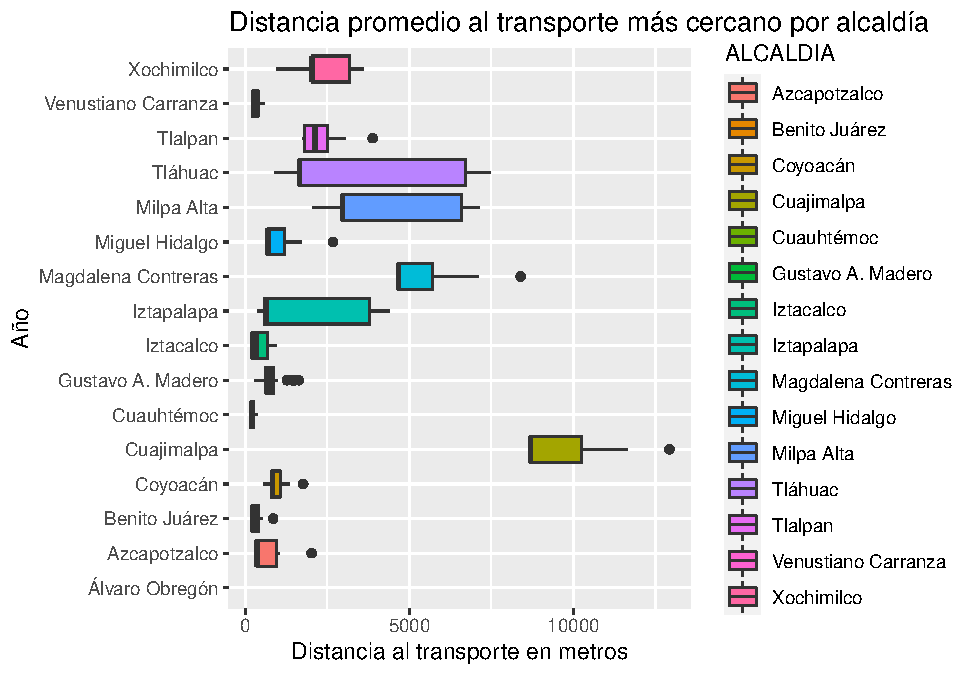
\includegraphics{proyecto_files/figure-latex/unnamed-chunk-6-1} \end{center}

\begin{center}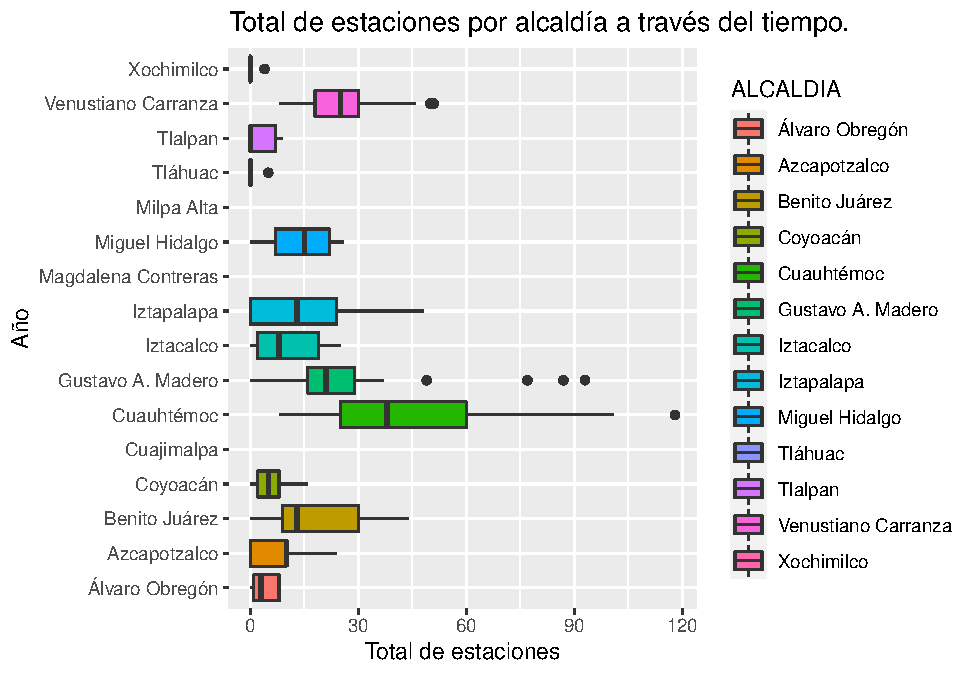
\includegraphics{proyecto_files/figure-latex/unnamed-chunk-7-1} \end{center}

\begin{center}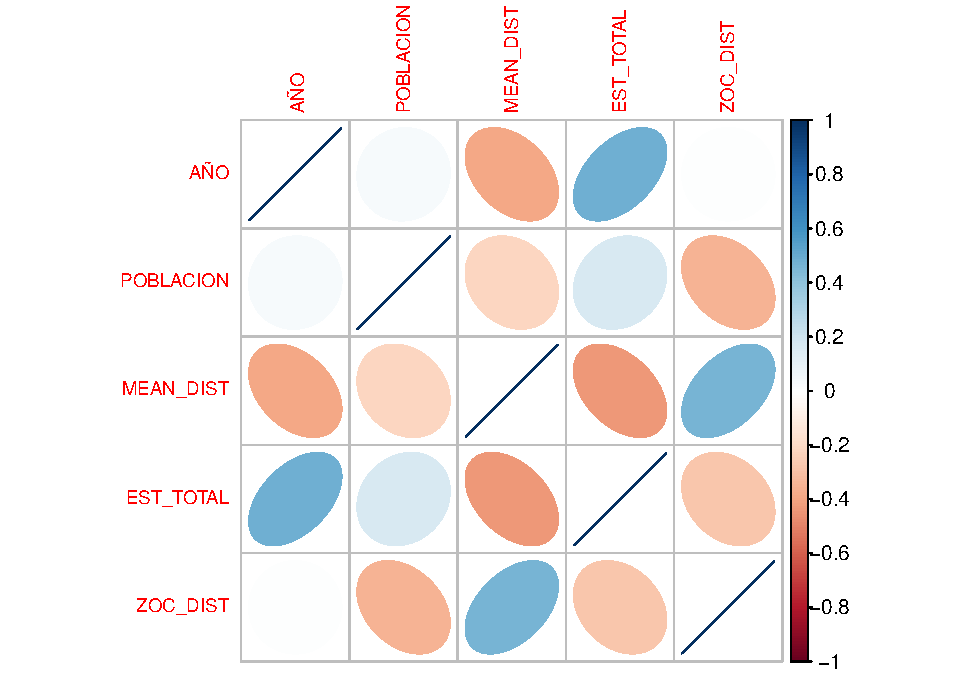
\includegraphics{proyecto_files/figure-latex/unnamed-chunk-8-1} \end{center}

\begin{center}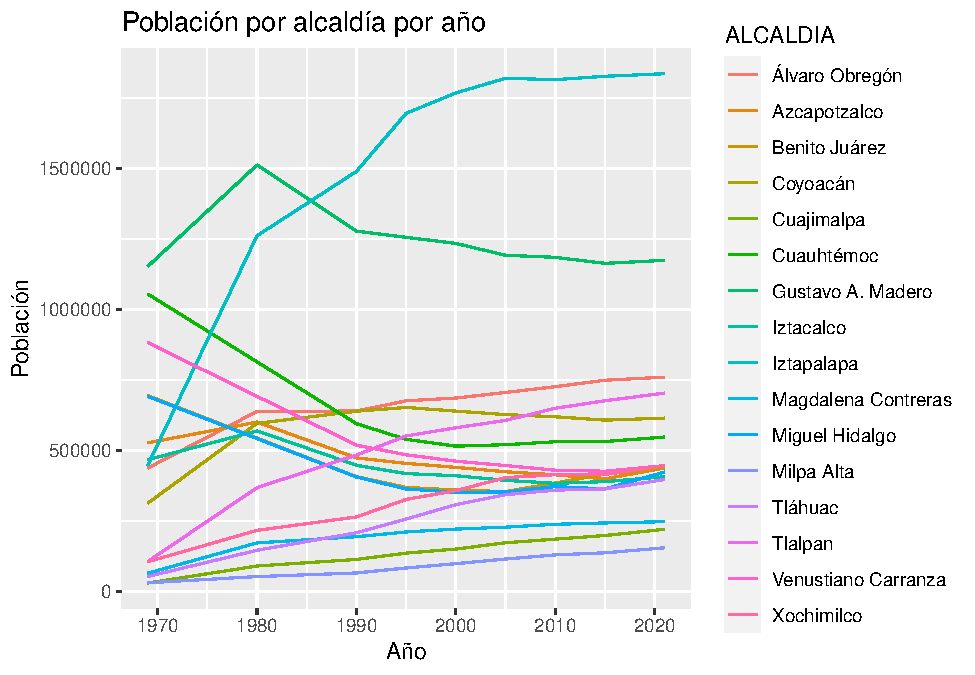
\includegraphics{proyecto_files/figure-latex/unnamed-chunk-9-1} \end{center}

\hypertarget{pca}{%
\subsection{PCA}\label{pca}}

\hypertarget{correlaciuxf3n-canuxf3nica}{%
\subsection{Correlación canónica}\label{correlaciuxf3n-canuxf3nica}}

\hypertarget{analisis-factorial}{%
\subsection{Analisis Factorial}\label{analisis-factorial}}

\hypertarget{pruebas-de-hipuxf3tesis}{%
\subsubsection{Pruebas de hipótesis}\label{pruebas-de-hipuxf3tesis}}

\hypertarget{regresiuxf3n-lineal}{%
\subsection{Regresión lineal}\label{regresiuxf3n-lineal}}

\hypertarget{interpretaciuxf3n-conclusiones-etc}{%
\subsection{Interpretación, conclusiones,
etc\ldots{}}\label{interpretaciuxf3n-conclusiones-etc}}

\end{document}
